\section{Applications}

\subsection{Stochastic Gradient Descent}

Here we consider $h(\mathbf{x}) = -\nabla f(\mathbf{x})$, and we track the ODE
\[
    \dot{\mathbf{x}}(t) = -\nabla f(\mathbf{x}(t)).
\]
With `rich noise', we have almost sure convergence to a local minimum if equilibria are isolated. (In general, pointwise convergence is not obvious but it holds for real analytic $f$). But, any isolated local minimum is a possible equilibrium with positive probability. This iterative scheme can slow down near saddle points. In this case, we can use momentum to accelerate the algorithm. That is, we use the iteration
\[
    \mathbf{x}_{n+1} = \mathbf{x}_n + \underbrace{a(n) \left[ -\nabla f(\mathbf{x}_n) + M_{n+1} \right]}_{\text{stochastic gradient term}} + \underbrace{b(n) \left[ \mathbf{x}_n - \mathbf{x}_{n-1} \right]}_{\text{momentum term}}.
\]
We may rewrite this as
\begin{align*}
    \mathbf{x}_{n+1} &= \mathbf{x}_n + \mathbf{y}_n \\
    \mathbf{y}_{n+1} &= \mathbf{y}_n - (1-b(n))\mathbf{y}_n + a(n) \left[ -\nabla f(\mathbf{x}_n) + M_{n+1} \right].
\end{align*}
This is reminiscent of the second order ODE
\[
    \dot{\mathbf{x}}(t) = \mathbf{y}(t), \quad \dot{\mathbf{y}}(t) = -\alpha \mathbf{y}(t) - \nabla f(\mathbf{x}(t)).
\]
Intuitively, this momentum scheme emulates Newton's laws with friction in a potential well. This allows the iterate to speed up near unstable critical points and on flat landscapes, and allows it to escape shallow valleys. This scheme helps in neural network training since the composition of sigmoidal functions often leads to flat patches. Note that we are not claiming that the iterate converges to the global minimum. It is entirely possible that there is a deep enough local minimum such that the momentum of the iterate is not enough for it to escape this minimum. However, the iterate automatically avoids irrelevant shallow minima. Moreover, this method avoids zigzagging in `pinched' landscapes, such as the rain-gutter landscape, shown below in Figure \ref{fig:raingutter}.

\begin{figure}[!ht]
    \centering
    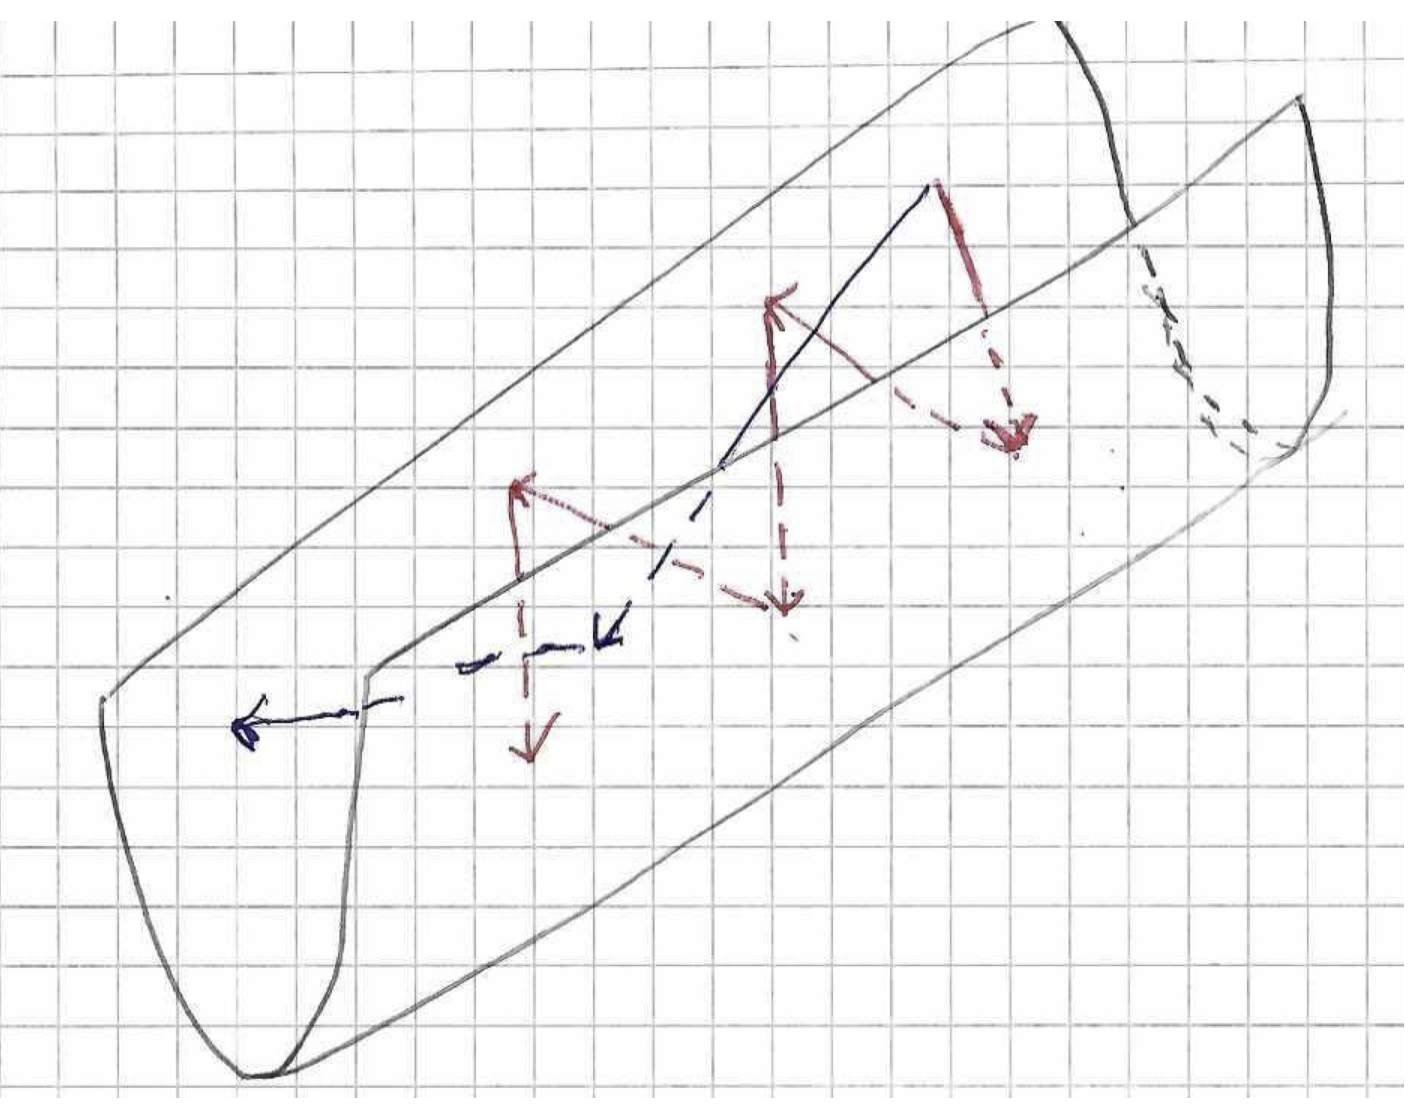
\includegraphics[width=0.7\linewidth]{raingutter.png}
    \caption{An example of a `pinched' landscape often called a rain-gutter landscape. Using traditional stochastic gradient descent, our iterate zigzags along the landscape (maroon trajectory), whereas adding momentum avoids this phenomenon (black trajectory)}
    \label{fig:raingutter}
\end{figure}
\newpage

There are more sophisticated variants such as Nesterov's accelerated gradient method. 

Typically, we do not have access to the gradient explicitly, and we must use an approximation. Sometimes, we may also be reluctant to evaluate the function too often since the evaluation procedure may be expensive. We now look at some approximation schemes. 

\begin{enumerate}
    \item \textbf{Kiefer-Wolfowitz.} This scheme uses finite difference approximations as:
    \begin{align*}
        \frac{\partial f}{\partial x_i}(\mathbf{x}) &\approx \frac{f(\mathbf{x} + \delta \mathbf{e}_i) - f(\mathbf{x})}{\delta} \\
        \frac{\partial f}{\partial x_i}(\mathbf{x}) &\approx \frac{f(\mathbf{x} + \delta \mathbf{e}_i) - f(\mathbf{x} - \delta \mathbf{e}_i)}{2\delta}
    \end{align*}
    These require $d+1$ and $2d$ function evaluations respectively. The discretisation error in the latter is better but it requires more function evaluations. 
    
    \item \textbf{Simultaneous perturbation (Spall).} We take $\Delta_n(i)$ ($n \geq 0$, $1 \leq i \leq d$) to be i.i.d. $\pm 1$ with equal probability. We set $\Delta_n \vcentcolon= \left( \Delta_n(1) , \ldots, \Delta_n(d) \right)$. Then, 
    \begin{align*}
        \frac{\partial f}{\partial x_i}(\mathbf{x}) &\approx \frac{f(\mathbf{x} + \delta \Delta_n) - f(\mathbf{x})}{\delta \Delta_n(i)} \\
        &\approx \frac{\partial f}{\partial x_i}(\mathbf{x}) + \sum_{j \neq i} \frac{\partial f}{\partial x_j} \frac{\Delta_n(j)}{\Delta_n(i)}.
    \end{align*}
    The second term can be absorbed into $M_{n+1}$. We may also use a single function estimate as follows.
    \begin{align*}
        \frac{\partial f}{\partial x_i}(\mathbf{x}) &\approx \frac{f(\mathbf{x} + \delta \Delta_n)}{\delta \Delta_n(i)} \\
        &= \frac{f(\mathbf{x})}{\delta \Delta_n(i)} + \frac{\partial f}{\partial x_i}(\mathbf{x}) + \sum_{j \neq i} \frac{\partial f}{\partial x_j} \frac{\Delta_n(j)}{\Delta_n(i)}.
    \end{align*}
    Here, both the first and third term can be absorbed into $M_{n+1}$. This scheme has numerical issues for small $\delta$ (small divisor problem). 
    
    \item \textbf{Flaxman-Kalai-McMahan.} We pick $\xi_n \in \mathbb{R}^d$ to be i.i.d. with zero mean and identity covariance matrix. Then, 
    \begin{align*}
        f_i(\mathbf{x} + \delta \xi_n) \xi_n(i) &\approx f_i(\mathbf{x})\xi_n(i) + \delta \frac{\partial f}{\partial x_i}(\mathbf{x}) \xi_n(i)^2 + \delta \sum_{j \neq i} \frac{\partial f}{\partial x_i}(\mathbf{x}) \xi_n(j) \xi_n(i) \\
        &= \delta \frac{\partial f}{\partial x_i}(\mathbf{x}) + f_i(\mathbf{x})\xi_n(i) + \delta \frac{\partial f}{\partial x_i}(\mathbf{x}) (\xi_n(i)^2-1) + \delta \sum_{j \neq i} \frac{\partial f}{\partial x_i}(\mathbf{x}) \xi_n(j) \xi_n(i) \\
        &= \delta \frac{\partial f}{\partial x_i}(\mathbf{x}) + \text{martingale difference terms}.
    \end{align*}
    
    \item \textbf{Mukherjee-Zhao.} To evaluate the gradient at $\mathbf{x}_0$, we recall that for $\mathbf{x}$ in a neighbourhood of $\mathbf{x}_0$, we have
    \[
        f(\mathbf{x}) \approx f(\mathbf{x}_0) + \left\langle \nabla f(\mathbf{x}_0), \mathbf{x} - \mathbf{x}_0 \right\rangle.
    \]
    We sample points $\mathbf{x}_i$, $1 \leq i \leq n$, in a neighbourhood of $\mathbf{x}_0$. Then, 
    \[
        \nabla f(\mathbf{x}_0) \approx \argmin_{\mathbf{y}} \sum_{m=1}^n \mathcal{K}(\mathbf{x}_m, \mathbf{x}_0) \cdot \left( f(\mathbf{x}_m) - f(\mathbf{x}_0) - \left\langle \mathbf{y}, \mathbf{x} - \mathbf{x}_0 \right\rangle \right)^2,
    \]
    where $\mathcal{K} \colon \mathbb{R}^d \times \mathbb{R}^d \to [0,\infty)$ is a suitable kernel function that satisfies $\mathcal{K}(\mathbf{x}, \mathbf{y}) \to 0$ as $\norm{\mathbf{x-y}} \to \infty$. 
    
    \item \textbf{Katkovnik-Kulchitsky.} Consider a Gaussian $g_{\sigma}(\cdot)$ with zero mean and variance $\sigma^2$. Then, for small $\sigma$, we can express $f(x)$ as a convolution with $g_{\sigma}$. That is,
    \[
        f(x) \approx \int g_{\sigma}(x-y) \cdot f(y) \, \D y.
    \]
    This gives us
    \[
        \nabla f(x) \approx \int \nabla g_{\sigma}(x-y) \cdot f(y) \, \D y,
    \]
    which is still a Gaussian expectation and can be estimated using Monte Carlo simulation. This scheme is particularly useful when $f$ is not differentiable to begin with. This scheme again has the small divisor problem for small $\sigma$, which can be ameliorated by additional averaging. 
\end{enumerate}

We also have a simulation-based optimisation paradigm, where we want to minimise $\E_{\theta} [f(X)]$ ($X$ is a real valued random variable) over $\theta$ where $\theta$ parameterises the distribution of $X$. We generate i.i.d. $X_n = \Phi(U_n, \theta)$ with the law corresponding to $\theta$ with $\{U_n\}$ uniform on $[0,1]$. Suppose $\Phi$ is continuously differentiable. We do
\[
    \theta_{n+1} = \theta_n - a(n) \cdot \frac{\partial}{\partial \theta} f\left( \Phi(U_{n+1}, \theta) \right) \bigg\rvert_{\theta = \theta_n}.
\]
A more sophisticated version is the likelihood ratio method, due to Glynn. Suppose the distributions $P_{\theta}$ corresponding to $\theta$ have densities with respect to a base distribution $P_{\theta_0}$. Let $\Lambda_{\theta}$ denote the likelihood ratio of $P_{\theta}$ with respect to $P_{\theta_0}$. Then, $\E_{\theta} [f(X)] = \E_{\theta_0}[f(X) \Lambda_{\theta}(X)]$. The algorithm then is
\[
    \theta_{n+1} = \theta_n - a(n)\cdot f(X_{n+1})\cdot \nabla_{\theta} \Lambda_{\theta}(X_{n+1}) \bigg\rvert_{\theta = \theta_n}.
\]

For global minimisation, we use the simulated annealing method, given by
\[
    \mathbf{x}_{n+1} = \mathbf{x}_n + a(n) \left[ - \nabla f(\mathbf{x}_n) + M_{n+1} \right] + b(n) W_{n+1}
\]
where $b(n) > 0$ is chosen appropriately given $\{a(n)\}$, and $\{W_n\}$ are i.i.d. $\mathcal{N}(0,1)$. This tracks the stationary distribution of the stochastic differential equation
\[
    \D X(t) = - \nabla f(X(t)) \, \D t + \frac{C}{\log T} \, \D B(t)
\]
as $T = t \uparrow \infty$, which asymptotically concentrates on the global minima of $f$. If we choose $a(n) = \frac{1}{n}$, then we choose $b(n) = \frac{C}{\sqrt{n\log\log n}}$.

\subsection{Stochastic Gradient Descent for Machine Learning}

Here, we are given samples of input-output pairs $(\mathbf{X}_n, \mathbf{Y}_n)$, $n \geq 1$. We wish to minimise the `empirical risk', given by
\[
    \frac{1}{N} \sum_{m=1}^N \mathcal{L} (\mathbf{X}_m, \mathbf{Y}_m, \Theta) \approx \E_{\Theta}[\mathcal{L}(\mathbf{X}_n, \mathbf{Y}_n, \Theta)].
\]
To replace the expectation by an average, we need the uniform strong law of large numbers. Sufficient conditions for these are given by the Vapnik-Chervonenkis theory and its extensions. Our target is to get sufficiently close to the minimum risk. That is, we want
\[
    \E \left[ \mathcal{L}(\mathbf{X}_n, \mathbf{Y}_n, \Theta_n) \right] \leq \min_{\Theta} \E\left[ \mathcal{L}(\mathbf{X}_n, \mathbf{Y}_n, \Theta) \right] + \epsilon
\]
for $0 < \epsilon \ll 1$. 

There are many special purpose variants of this, such as mini-batch algorithms, ADAGRAD, ADAM. Sometimes, the number of samples is large enough to be comparable to the ambient space. A typical fix for this is to use block-coordinate descent. 

\subsection{Gradient Ascent-Descent}

For $f(\cdot, \mathbf{y})$ convex and $f(\mathbf{x},\cdot)$ concave (with at least one of them strict), consider the coupled ODEs
\begin{align*}
    \dot{\mathbf{x}}(t) &= -\nabla_{\mathbf{x}} f\left( \mathbf{x}(t), \mathbf{y}(t) \right) \\
    \dot{\mathbf{y}}(t) &= \nabla_{\mathbf{y}} f\left( \mathbf{x}(t), \mathbf{y}(t) \right).
\end{align*}
Here, we take $V(\mathbf{x}, \mathbf{y}) = \norm{\mathbf{x-x}^*}^2 + \norm{\mathbf{y-y}^*}^2$ where $(\mathbf{x}^*,\mathbf{y}^*)$ is a saddle point. Then, 
\begin{align*}
    \frac{\D}{\D t} V(\mathbf{x},\mathbf{y}) &= - \left\langle \mathbf{x}(t) - \mathbf{x}^*, \nabla_{\mathbf{x}} f(\mathbf{x}(t),\mathbf{y}(t)) \right\rangle + \left\langle \mathbf{y}(t) - \mathbf{y}^*, \nabla_{\mathbf{y}} f(\mathbf{x}(t),\mathbf{y}(t)) \right\rangle \\
    &\leq \left( f(\mathbf{x}*,\mathbf{y}(t)) - f(\mathbf{x}(t),\mathbf{y}(t)) \right) + \left( f(\mathbf{x}(t),\mathbf{y}(t)) - f(\mathbf{x}(t),\mathbf{y}^*) \right) \\
    &= \left( f(\mathbf{x}*,\mathbf{y}(t)) - f(\mathbf{x}(t),\mathbf{y}^*) \right) + \left( f(\mathbf{x}(t),\mathbf{y}^*) - f(\mathbf{x}(t),\mathbf{y}^*) \right) \\
    &\leq 0
\end{align*}
with strict inequality away from the saddle point. Thus, this is a Liapunov function. This is particularly useful for primal-dual methods for the problem 
\[
    \text{minimise } f(\mathbf{x}) \quad \text{subject to} \quad g(\mathbf{x}) \leq C.
\]
Here, we do
\begin{align*}
    \mathbf{x}_{n+1} &= \mathbf{x}_n - a(n) \left[ \nabla f(\mathbf{x}_n) + \bm{\lambda}_n^{\top} \nabla g(\mathbf{x}_n) + M_{n+1} \right] \\
    \bm{\lambda}_{n+1} &= \bm{\lambda}_n + a(n) \left[ g(\mathbf{x}_n) - C\right]. 
\end{align*}
Here, we descend along $\mathbf{x}$ and ascend along $\bm{\lambda}$. We are seeking the saddle point of the Lagrangian, defined as
\[
    \mathcal{L}(\mathbf{x},\bm{\lambda}) \vcentcolon= f(\mathbf{x}) + \bm{\lambda}^{\top} (g(\mathbf{x}) - C). 
\]
Thus, we have
\begin{align*}
    \nabla_{\mathbf{x}} \mathcal{L}(\mathbf{x}, \bm{\lambda}) &= \nabla f(\mathbf{x}) + \bm{\lambda}^{\top} \nabla g(\mathbf{x}) \\
    \nabla_{\bm{\lambda}} \mathcal{L}(\mathbf{x}, \bm{\lambda}) &= g(\mathbf{x}) - C. 
\end{align*}

\subsection{Fixed Point Schemes}

Suppose $F \colon \mathbb{R}^d \to \mathbb{R}^d$ is Lipschitz. We wish to find a fixed point of $F$, that is, we wish to find $\mathbf{x}^*$ such that $F(\mathbf{x}^*) = \mathbf{x}^*$. Suppose $F$ is a contraction map. That is, for one of
\[
    \norm{\mathbf{x}}_p \vcentcolon= \left( \sum_{i=1}^d \abs{x_i}^p \right)^{\frac{1}{p}}, 1 \leq p < \infty \quad \norm{\mathbf{x}}_{\infty} \vcentcolon= \max_i \abs{x_i},
\]
we have
\[
    \norm{F(\mathbf{x}) - F(\mathbf{y})}_p \leq \alpha \norm{\mathbf{x} - \mathbf{y}}_p \quad \forall \mathbf{x,y},
\]
where $0 < \alpha < 1$. Then, there is a unique fixed point $\mathbf{x}^*$ and $\mathbf{x}_n \to \mathbf{x}^*$ almost surely. In this case, $V(\mathbf{x}) \vcentcolon= \norm{\mathbf{x} - \mathbf{x}^*}_p$ works as a Liapunov function. 

This also works 
\begin{enumerate}
    \item \emph{Weighted norms.} 
    \[
        \norm{\mathbf{x}}_{\mathbf{w},p} \vcentcolon= \left( \sum_{i=1}^d w_i \abs{x_i}^p \right)^{\frac{1}{p}}
    \]
    \item \emph{Pseudo-contractions.} 
    \[
        \norm{F(\mathbf{x}) - F(\mathbf{x}^*)}_p \leq \alpha \norm{\mathbf{x} - \mathbf{x}^*}_p \quad \forall \mathbf{x},
    \]
    where $\mathbf{x}^*$ is the fixed point, $0 < \alpha < 1$, and $1 < p \leq \infty$. 
    
    \item \emph{Anti-monotone $f$.} 
    \[
        \left\langle F(\mathbf{x}) - F(\mathbf{y}), \mathbf{y} - \mathbf{x} \right\rangle < 0 \quad \text{for } \mathbf{x} \neq \mathbf{y}.
    \]
    The above inequality also generalises monotonicity to higher-dimensional and more general spaces. 
    
    \item \emph{Special cases of `non-expansive' maps.} 
    \[
        \norm{F(\mathbf{x}) - F(\mathbf{y})} \leq  \norm{\mathbf{x} - \mathbf{y}} \quad \forall \mathbf{x,y}.
    \]
\end{enumerate}

\subsection{Replicator Dynamics}

This is an application in the field of evolutionary biology and evolutionary game theory where the iterates are in the probability simplex. We have
\begin{equation*}
    \dot{p}_i(t) = p_i(t) f_i(\mathbf{p}(t)) - \sum_{j} p_j(t) f_j(\mathbf{p}(t)) \tag{$\star$}
\end{equation*}
Here, $p_i(t)$ is the fraction of species $i$ at time $t$ and $f_i(\mathbf{p})$ denotes the payoff to species $i$ if the current population profile is $\mathbf{p}$. Thus, if the payoff for species $i$ is higher than average, then the fraction of species $i$ increases. The probability simplex
\[
    \mathcal{S} \vcentcolon= \left\{ \mathbf{x} = [x_1, \ldots, x_d] \in \mathbb{R}^d \colon x_i \geq 0 \, \forall i \,  \sum_ix_i = 1 \right\}
\]
is invariant under $(\star)$, as are its faces corresponding to one or more $x_i = 0$. The stable equilibria here correspond to `evolutionary stable equilibria', that is, equilibria that are stable under single mutations. 

The above iterates converge, for example, if $f_i = \frac{\partial F}{\partial x_i}$, in which case this is called a `potential game' with potential $F$. In this case, we take $V = -F$. We have
\[
    \frac{\D}{\D t} F(\mathbf{x}(t)) = \sum_i p_i(t) \left( \frac{\partial F}{\partial x_i}(\mathbf{p}(t)) \right)^2 - \left( \sum_i p_i(t) \frac{\partial F}{\partial x_i}(\mathbf{p}(t)) \right)^2
\]
This is positive unless $\nabla F$ is a constant vector, in which case the gradient along the probability simplex $\mathcal{S}$ is zero. 